\clearpage

\begin{figure}[hbt!]
	\caption{Leftmost Stock Price Digit and Probability of Sale, Quarterly Sample}%
	\label{fig:left_digit_sell_main}%
	\centering%	
	\bigskip
	\subfigure[Price Increasing]{
		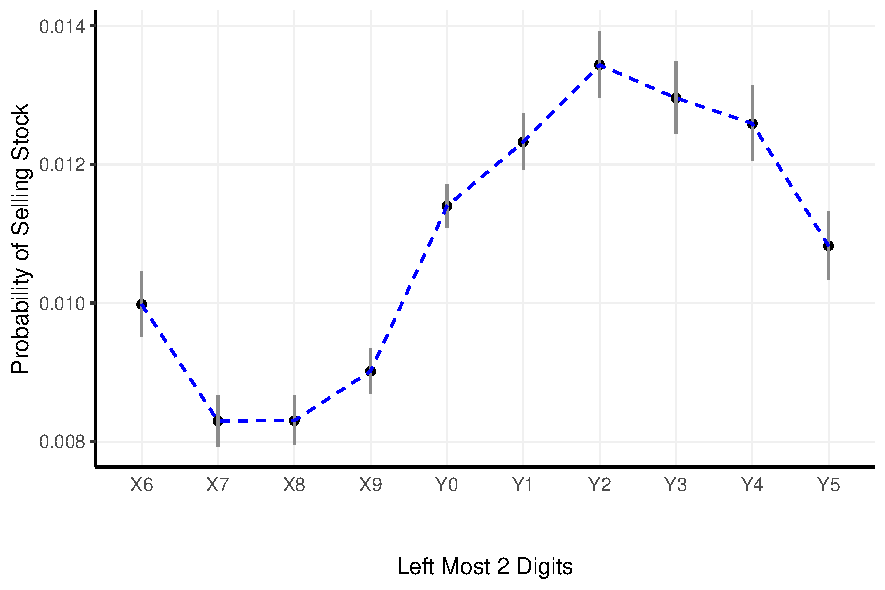
\includegraphics[width=0.45\textwidth]{figures/Left2increase_probCI_quarter.pdf}
		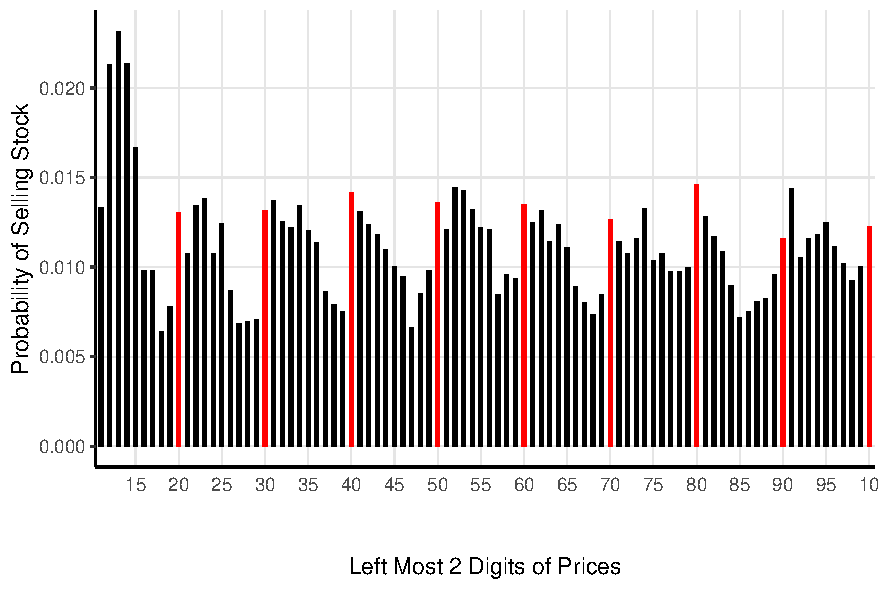
\includegraphics[width=0.45\textwidth]{figures/2left_increase_quarter.pdf}	
	}
	\subfigure[Price Decreasing]{
		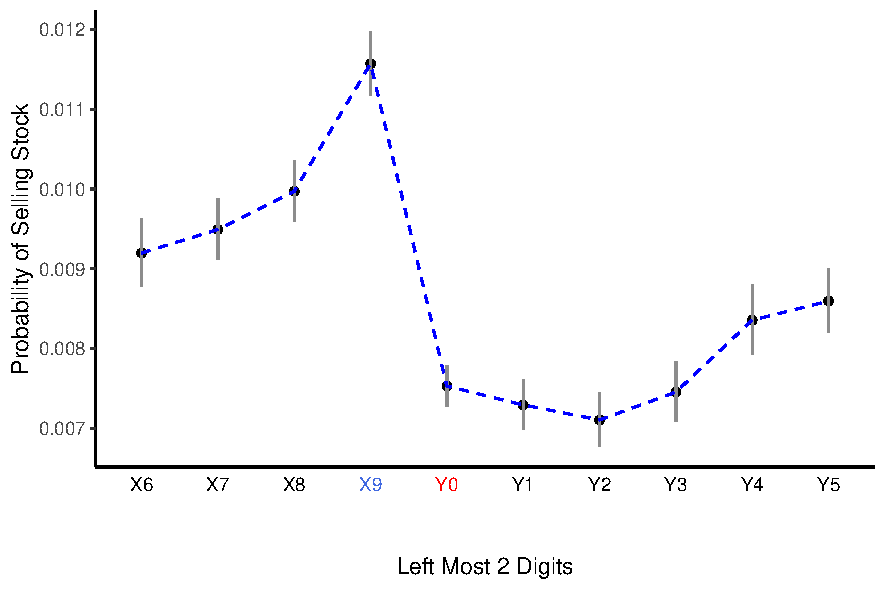
\includegraphics[width=0.45\textwidth]{figures/Left2decrease_probCI_quarter.pdf}
		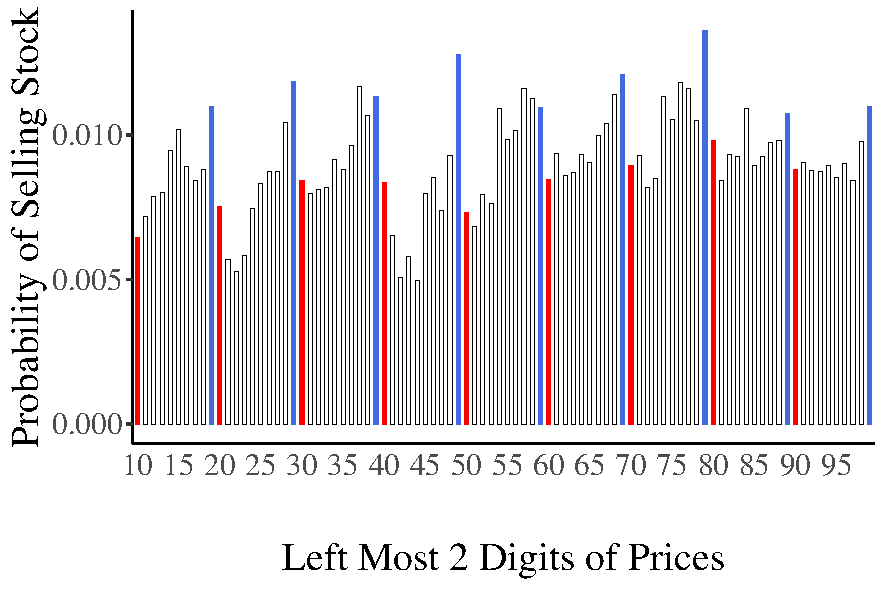
\includegraphics[width=0.45\textwidth]{figures/2left_decrease_quarter.pdf}	
	}
	\fignote{£$Y$ in the X-axes is equivalent to £$X+1$ (e.g., £X9 could include £0.19, £1.9, £19, etc., while £Y0 could include £0.20, £2.0, £20, etc.).}
\end{figure}

\clearpage

\begin{figure}[hbt!]
	\caption{Leftmost Stock Price Digit and Probability of Sale \\ Prices Increasing Sample by Price Range}%
	\label{fig:left_digit_sell_increase_main}%
	\centering%	
	\bigskip
	\subfigure[Price = \pounds0.11 to \pounds1.01]{
		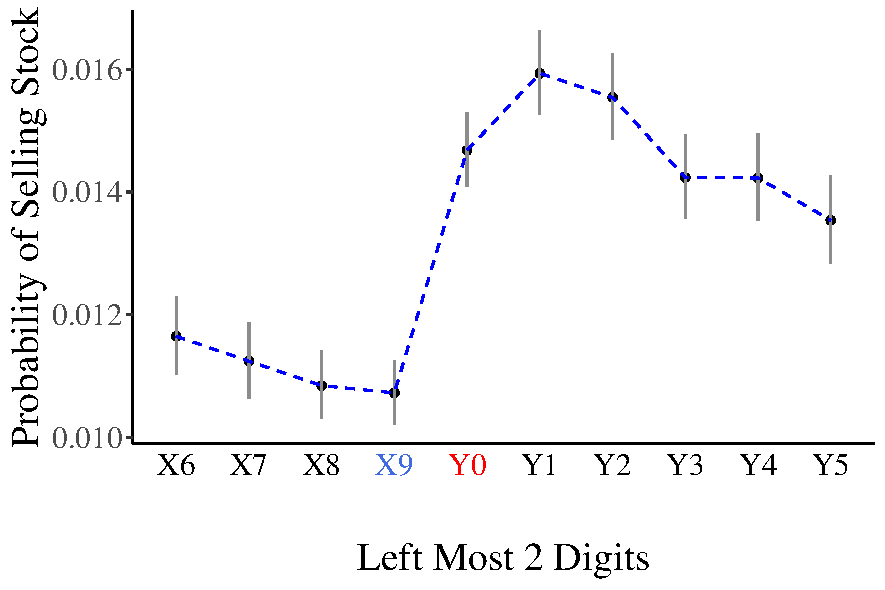
\includegraphics[width=0.45\textwidth]{figures/Left2increases_1pbin_CI_quarter.pdf}
		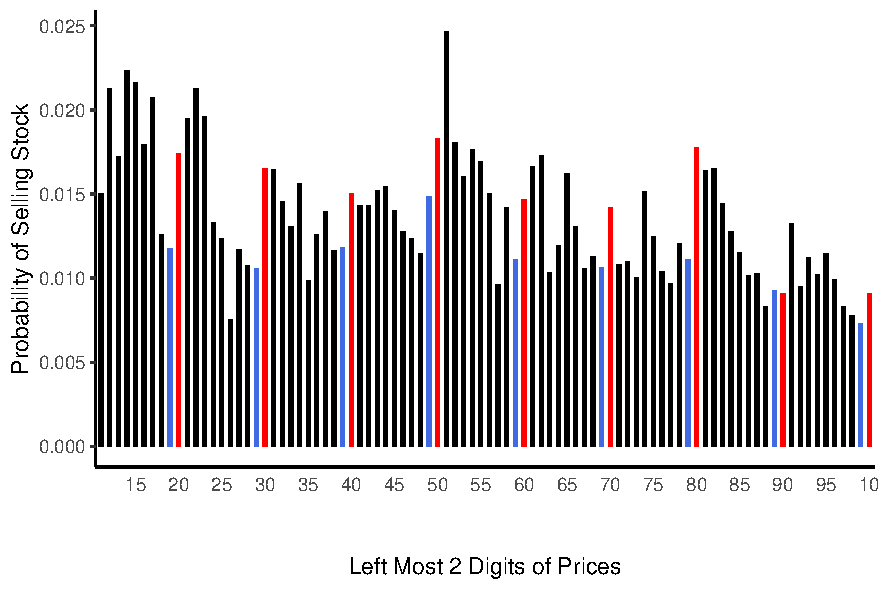
\includegraphics[width=0.45\textwidth]{figures/2left_increase_bin1p_quarter.pdf}
	}
	\subfigure[Price = \pounds1.01 to \pounds10.1]{
		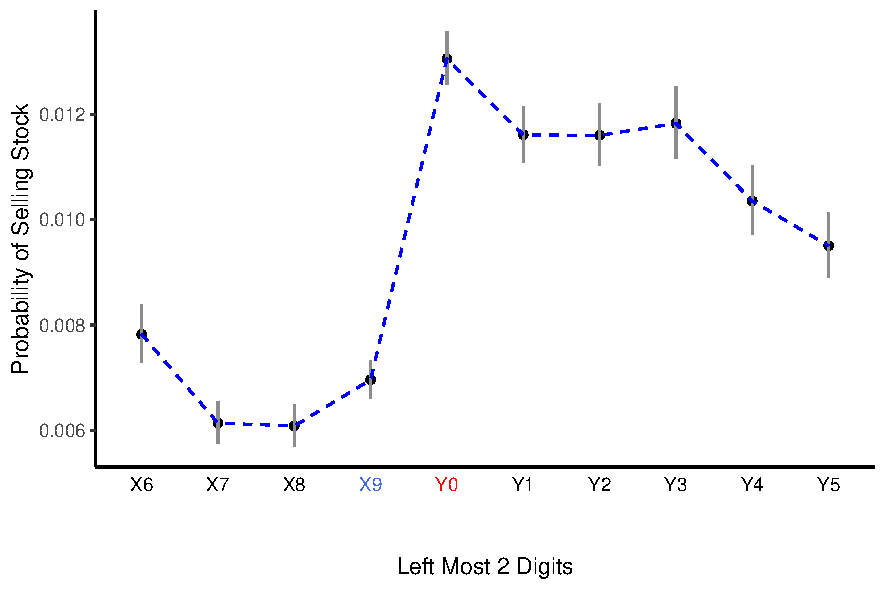
\includegraphics[width=0.45\textwidth]{figures/Left2increases_10pbin_CI_quarter.pdf}
		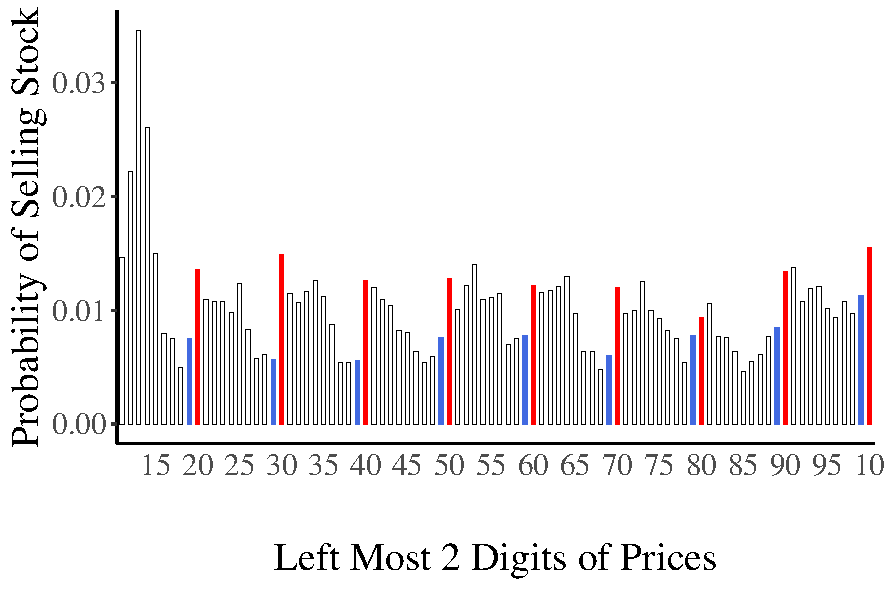
\includegraphics[width=0.45\textwidth]{figures/2left_increase_bin10p_quarter.pdf}
	}
	\subfigure[Price = \pounds11 to \pounds101]{
		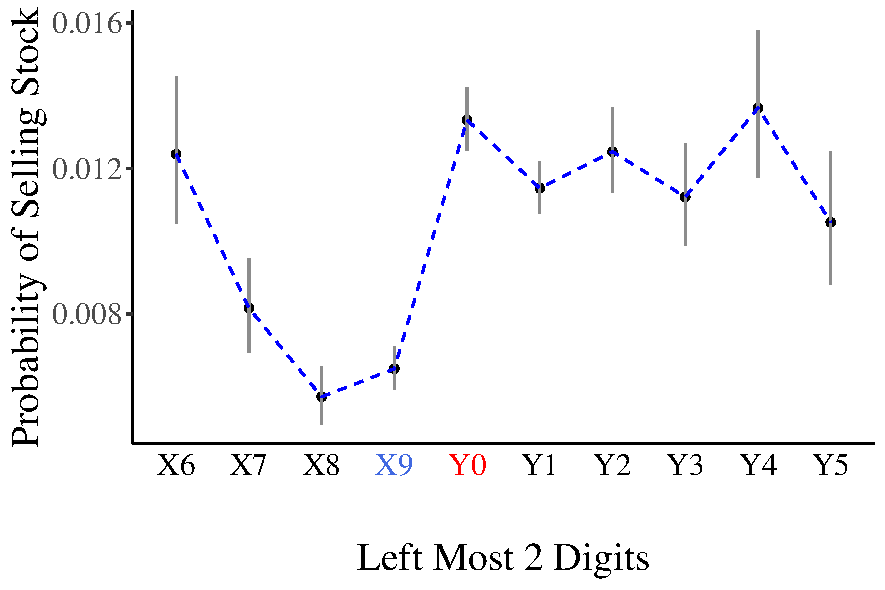
\includegraphics[width=0.45\textwidth]{figures/Left2increases_1poundbin_CI_quarter.pdf}
		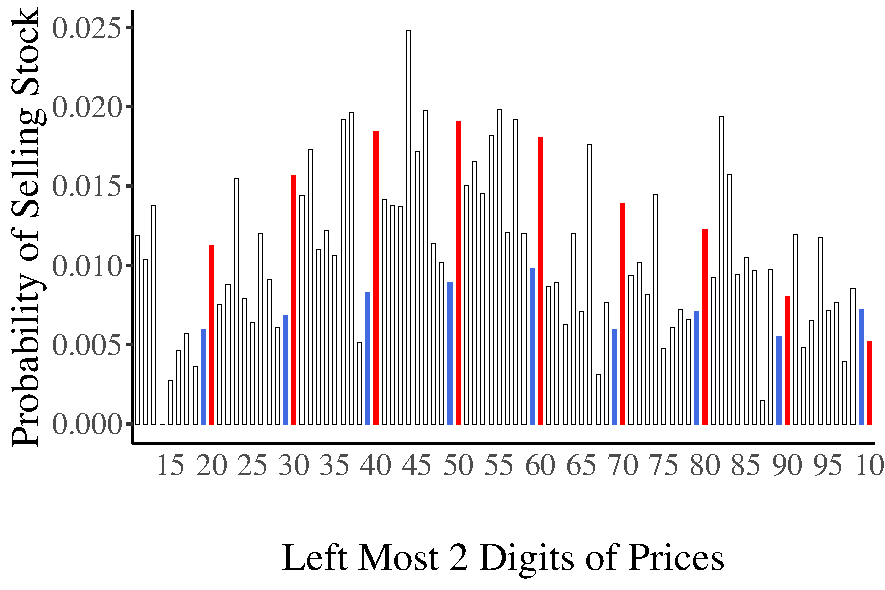
\includegraphics[width=0.45\textwidth]{figures/2left_increase_bin1pound_quarter.pdf}
	}
	\fignote{£$Y$ in the X-axes is equivalent to £$X+1$ (e.g., £X9 could include £0.19, £1.9, £19, etc., while £Y0 could include £0.20, £2.0, £20, etc.). Panels A, B and C show equal size bins of 1p, 10p and £1, respectively. Panel A corresponds to 25\% of the observations in the prices increasing sample; Panel B, to 55\%; and Panel C, to 8\%.}
\end{figure}

\clearpage
\begin{figure}[hbt!]
	\caption{Leftmost Stock Price Digit and Probability of Sale \\ Prices Decreasing Sample by Price Range}%
	\label{fig:left_digit_sell_decrease_main}%
	\centering%	
	\bigskip
	\subfigure[Price = \pounds0.10 to \pounds1.00]{
		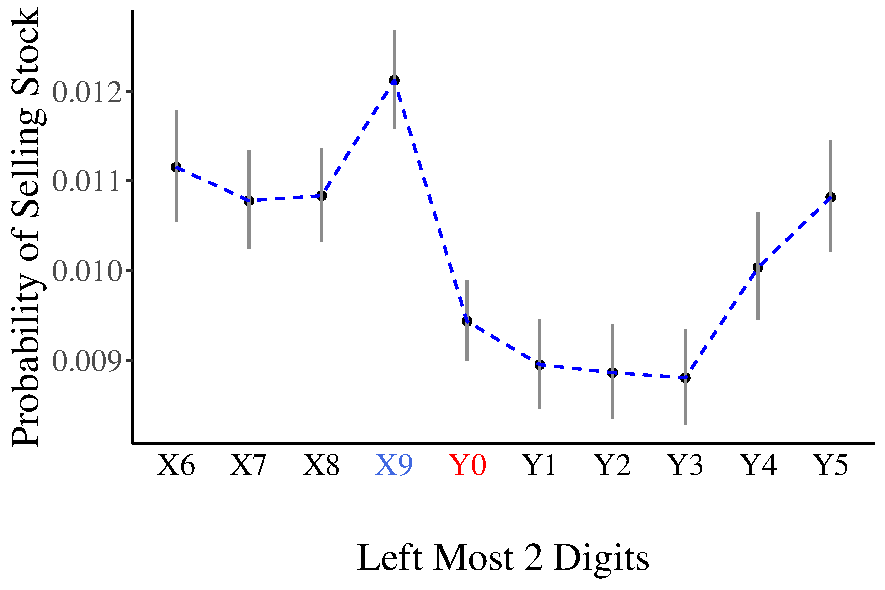
\includegraphics[width=0.45\textwidth]{figures/Left2decreases_1pbin_CI_quarter.pdf}
		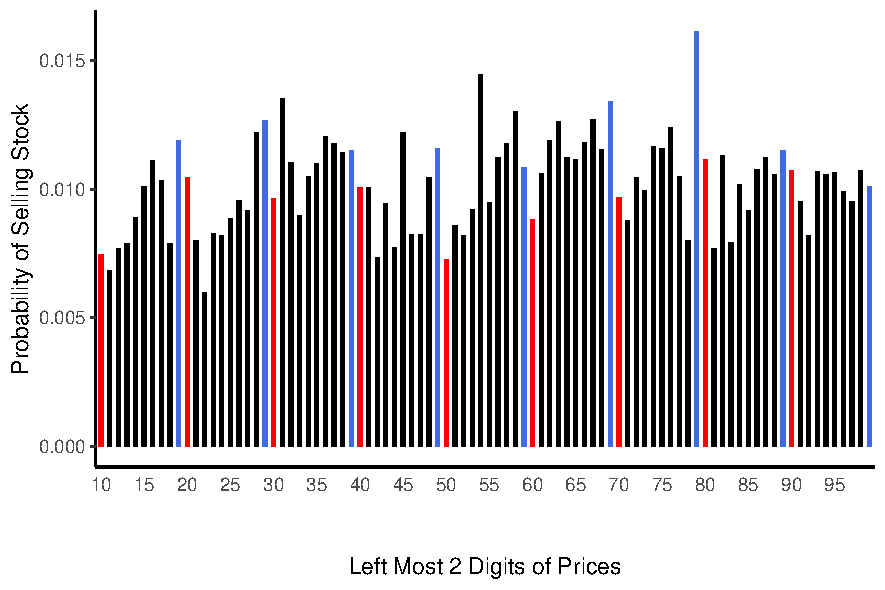
\includegraphics[width=0.45\textwidth]{figures/2left_decrease_bin1p_quarter.pdf}
	}
	\subfigure[Price = \pounds1.00 to \pounds10.0]{
		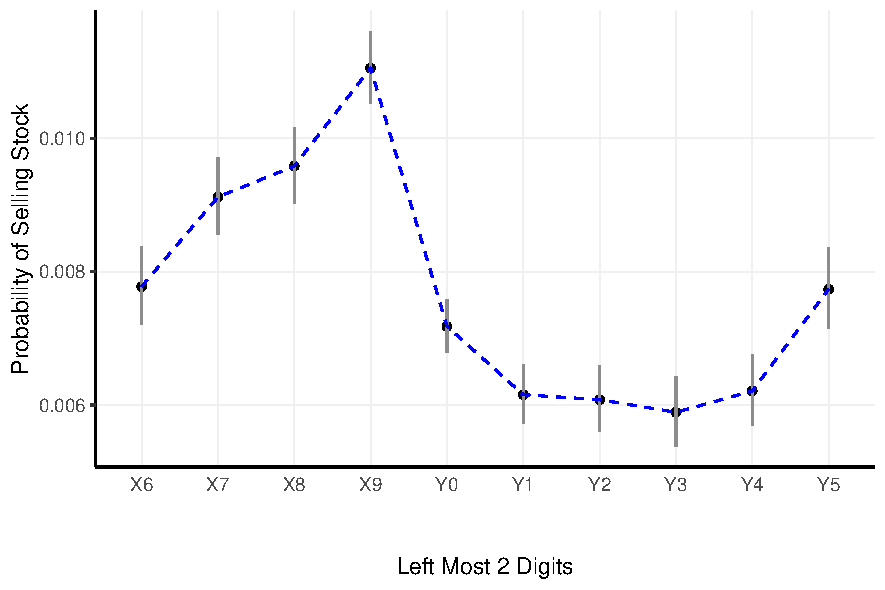
\includegraphics[width=0.45\textwidth]{figures/Left2decreases_10pbin_CI_quarter.pdf}
		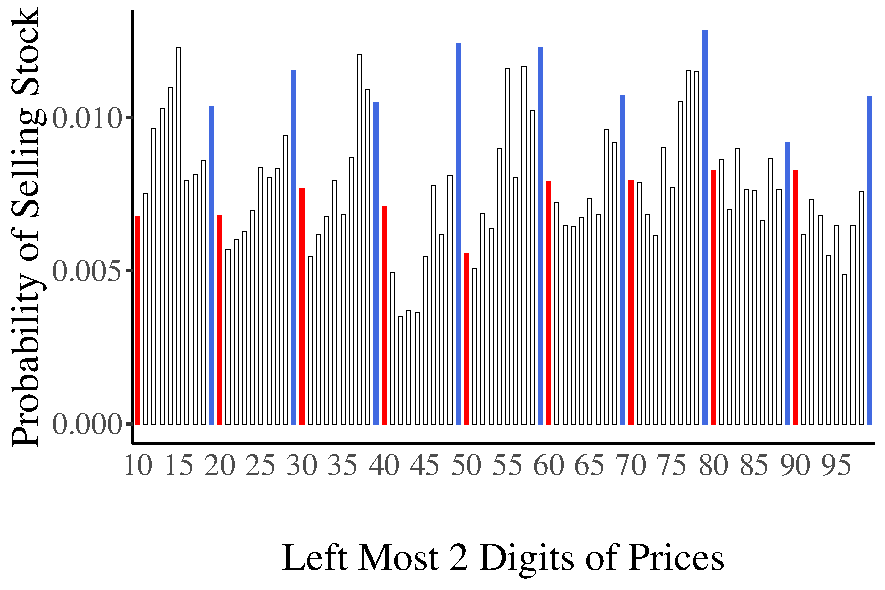
\includegraphics[width=0.45\textwidth]{figures/2left_decrease_bin10p_quarter.pdf}
	}
	\subfigure[Price = \pounds10 to \pounds100]{
		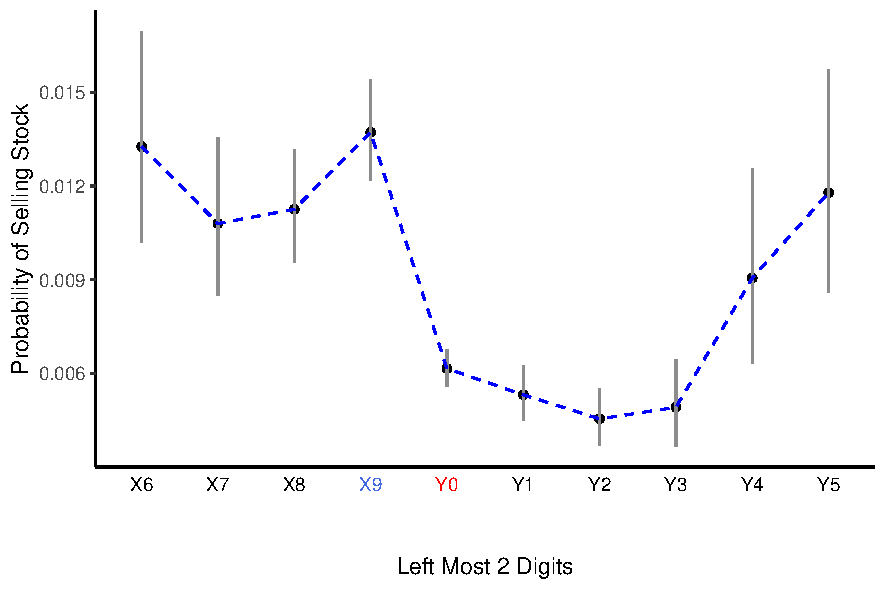
\includegraphics[width=0.45\textwidth]{figures/Left2decreases_1poundbin_CI_quarter.pdf}
		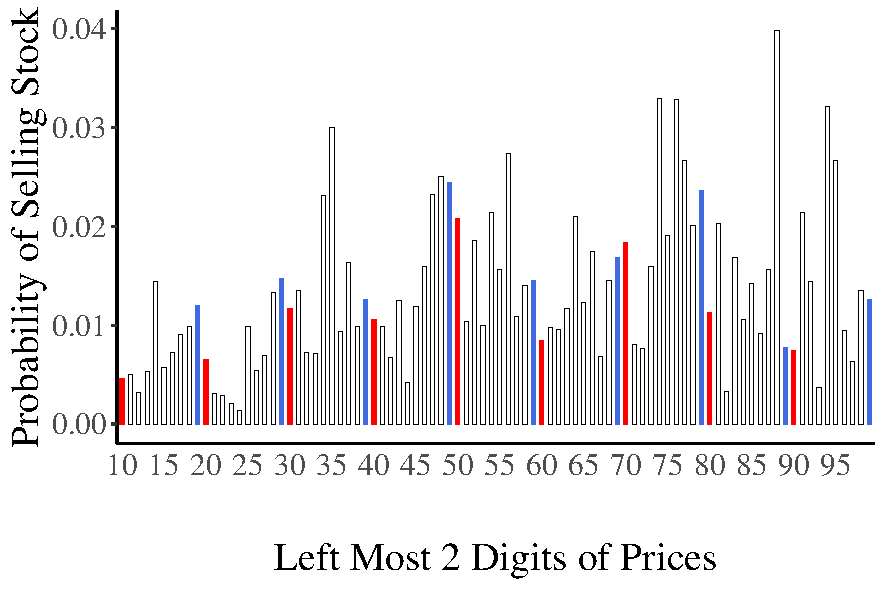
\includegraphics[width=0.45\textwidth]{figures/2left_decrease_bin1pound_quarter.pdf}
	}
	\fignote{£$Y$ in the X-axes is equivalent to £$X+1$ (e.g., £X9 could include £0.19, £1.9, £19, etc., while £Y0 could include £0.20, £2.0, £20, etc.). Panels A, B and C show equal size bins of 1p, 10p and £1, respectively. Panel A corresponds to 27\% of the observations in the prices decreasing sample; Panel B, to 43\%; and Panel C, to 7\%.}
\end{figure}